\documentclass[conference]{IEEEtran}
\IEEEoverridecommandlockouts
% The preceding line is only needed to identify funding in the first footnote. If that is unneeded, please comment it out.
\usepackage{cite}
\usepackage{amsmath,amssymb,amsfonts}
\usepackage{algorithmic}
\usepackage{graphicx}
\usepackage{textcomp}
\usepackage{xcolor}
\usepackage[english]{babel}
\usepackage{booktabs} % For improved table formatting
\usepackage{array} % For improved column formatting
\usepackage{multicol} % For multi-column formatting
\usepackage{url}

\def\BibTeX{{\rm B\kern-.05em{\sc i\kern-.025em b}\kern-.08em
    T\kern-.1667em\lower.7ex\hbox{E}\kern-.125emX}}
\begin{document}

\title{Securing Data in Low-Resource Environments: Lightweight Block Ciphers}


\author{\IEEEauthorblockN{Fernando Ramirez Arredondo}
\IEEEauthorblockA{\textit{Computer Science} \\
\textit{Universidad Católica San Pablo}\\
Arequipa, Perú \\
fernando.ramirez@ucsp.edu.pe}
\and
\IEEEauthorblockN{Yván Jesús Túpac Valdivia}
\IEEEauthorblockA{\textit{Computer Science} \\
\textit{Universidad Católica San Pablo}\\
Arequipa, Perú \\
ytupac@ucsp.edu.pe}}


\maketitle

\begin{abstract}
    Ensuring communication security for devices with limited resources is vital in the contemporary landscape. This work classifies seven state-of-the-art lightweight block ciphers designed for such devices. These ciphers offer efficient encryption for data security while minimizing resource consumption. Our analysis focuses on the two main categories of lightweight block ciphers, Substitution-Permutation Networks and Feistel Networks. We explore the key strategies these ciphers leverage to achieve state-of-the-art performance. In particular, the analysis reveals that two prominent techniques are employed, bit-slicing and structure modification. These techniques play a significant role in optimizing the ciphers for resource-constrained environments.
\end{abstract}

\begin{IEEEkeywords}
iot, feistel, substitution-permutation, resource-constrained, lightweight, cryptography
\end{IEEEkeywords}

\section{Introduction}

The Internet of Things (IoT) has spawned an era of interconnected devices, generating vast amounts of data and transforming our interaction with the physical world. This connectivity presents a growing security challenge when the devices generating or transmitting sensitive data lack the resources to perform up-to-standard encryption processes. As Thakor et al. \cite{IoT_1} categorize, IoT devices fall into two resource-based groups, resource-rich devices like servers, personal computers, and smartphones, and resource-constrained devices like sensor nodes, RFID tags, and actuators (Table \ref{table:crypto_devices}).

\begin{table}[ht]
    \centering
    \caption{Cryptographic Approaches on Different Devices\cite{IoT_1}}
    \begin{tabular}{ll}
        \toprule
        \textbf{Device} & \textbf{Cryptography} \\
        \midrule
        Servers, Desktops and Smartphones & Conventional Cryptography \\
        Embedded Systems and RFID & Lightweight Cryptography \\
        \bottomrule
    \end{tabular}
    \label{table:crypto_devices}
\end{table}

This challenge is further amplified by the evolution of IoT, which has transitioned from smaller networks to wide area networks, leading to a rapid growth in the number of interconnected devices. As IoT applications increase, a substantial amount of sensitive data is exchanged, raising concerns about privacy and security. Increased device interconnectivity further intensifies these concerns, potentially exposing new vulnerabilities with each additional device. In a landscape with billions of interconnected devices, even a single security flaw can be exploited on a massive scale.

Just as physical security measures like locks, safes, and opaque envelopes protect our valuables, cryptography serves as the digital equivalent, safeguarding the integrity and confidentiality of data in our online activities. This work aims to contribute to the application of cryptography for resource-constrained devices in the ever-expanding IoT landscape, where robust security solutions are essential to trust the activities and processes we reproduce or create from scratch in the digital world. 
Traditional cryptography, often computationally intensive, is impractical for these resource-constrained devices.  Lightweight cryptography emerges as a modern solution, specifically designed for devices with limitations in memory, processing power, and energy consumption. It prioritizes low computational complexity and a small memory footprint\cite{zhong2024lightweight}.

Traditional ciphers are categorized into two classes, asymmetric and symmetric. While asymmetric ciphers offer enhanced security features, they require greater computational resources and often have higher implementation costs. Consequently, they are less suitable for resource-constrained devices. Lightweight ciphers prefer the symmetric approach due to being generally faster and requiring less computational power. Following this same line of thinking, the vast majority of these ciphers are designed to operate on fixed-sized blocks of data rather than streams of data, as can be seen in NIST latest Lightweight Cryptography Standardization Process\cite{NIST}. It is for this reason that this study focuses on block ciphers, specifically on two fundamental structures employed in lightweight block ciphers, Feistel Networks and Substitution-Permutation Networks.

\begin{figure*}
    \centering
    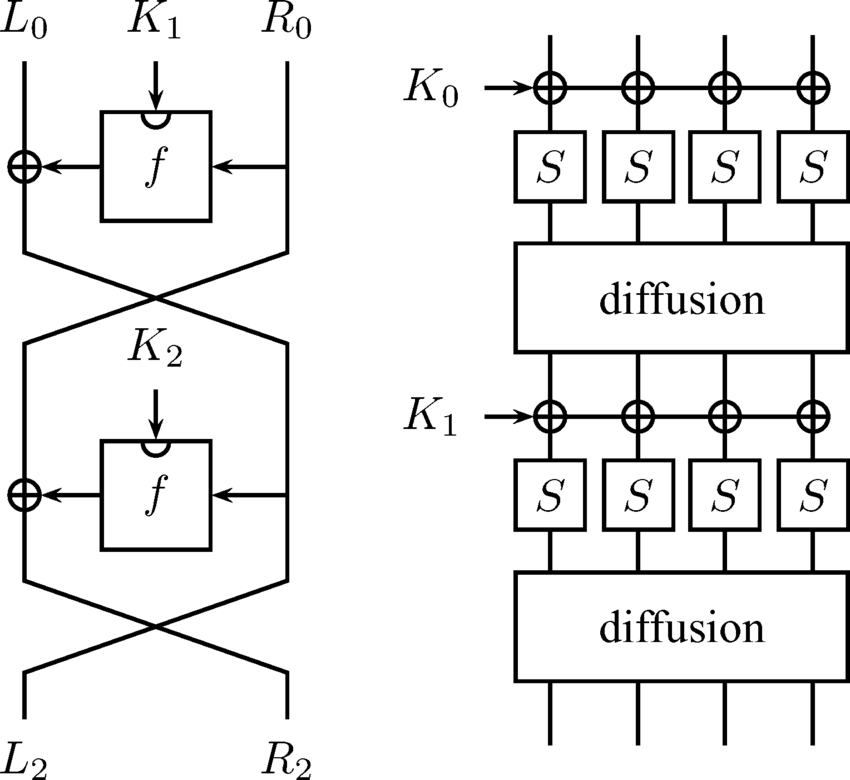
\includegraphics[width=\columnwidth]{figures/FEISTEL-SPN.png}
    \caption{Generalization of a Feistel Network (left) and a Substitution-Permutation Network (right)\cite{de2006introduction}.}
    \label{fig:FEISTEL-SPN}
\end{figure*}

The Feistel Network (FN) stands as a fundamental structure in block cipher design. It offers a modular and efficient approach to encryption, employing multiple rounds of data processing. In each round, a half-block of data is processed using a round function, often incorporating non-linear substitutions and permutations. The output of this function is then combined with the other half-block using an XOR operation, creating a dependency between rounds that improves the overall security\cite{FEISTEL}.

The Substitution-Permutation Network (SPN) is another block cipher structure. It relies on a series of substitution and permutation stages. Substitution box (S-box) replaces data bits with new values, introducing non-linearity to confuse potential attackers. Permutation box (P-box) rearranges the data bits, making it challenging to discern the original data\cite{heys1996substitution}. Refer to Fig.\ref{fig:FEISTEL-SPN} for a general view of both FN and SPN structures.

Both FN and SPN structures offer advantages in lightweight cryptography. FN structures are known for their modularity and ease of implementation, while SPN structures provide inherent parallelism, potentially leading to faster encryption/decryption on certain architectures.

\begin{table}[ht]
    \centering
    \caption{Table of Abbreviations}
    \begin{tabular}{ll}
        \toprule
        \textbf{Abbreviation} & \textbf{Definition} \\
        \midrule
        ASIC & Application-Specific Integrated Circuit \\
        DULBC & Dynamic Ultra-Lightweight Block Cipher \\
        FN & Feistel Network \\
        FPGA & Field-Programmable Gate Array \\
        IVLBC & InVolutive Lightweight Block Cipher \\
        IoT & Internet of Things \\
        KSA & Key Scheduling Algorithm \\
        LBC & Lightweight Block Cipher \\
        LBCCS & Lightweight Block encryption algorithm \\
        & based on Combined Chaotic System \\
        NIST & National Institute of Standards and Technology (USA) \\
        P-box & Permutation box \\
        RFID & Radio Frequency IDentification \\
        S-box & Substitution box \\
        SPN & Substitution-Permutation Network \\
        Ssb & Synthetic s-box \\
        $f$ & Function \\
        \bottomrule
    \end{tabular}
    \label{table:abbreviations}
\end{table}

This paper makes an exploration of FN and SPN structures in the context of lightweight cryptography. We will provide analysis of their design principles, operational workflows, and suitability for resource-constrained devices. Refer to Table \ref{table:abbreviations} for the full list of abbreviations.

\section{State of the art}

This section explores lightweight block ciphers, introducing them based on their structure and the techniques that generate their state-of-the-art performance for resource-constrained devices.

\subsection{SPN-based solutions}

Yang et al. introduced Dynamic Ultra-Lightweight Block Cipher (DULBC), a dynamic SPN structure in which the specific encryption process changes based on the round keys. DULBC utilizes a unique approach where the round function is not fixed. Each round selects one of four $f$s based on the first two bits of the round key, making it more resistant to attacks compared to static ciphers. This enhances security without significant hardware overhead. The proposed S-box offers good cryptographic properties with minimal cost. It consists of three NOR and XOR, one NAND and XNOR operations. leading to a simple inverse and efficient implementation. The authors highlight successful FPGA and ASIC implementations of DULBC, demonstrating its high throughput and relatively low area requirements. Security analysis confirms the resistance of DULBC to various attacks, including differential attacks, linear attacks, and side-channel attacks. In conclusion, DULBC presents a promising solution for resource-limited environments due to its dynamic structure, efficient S-box design, and strong security profile\cite{DULBC}.


Yasmin and Gupta proposed a modification to the LBC GIFT\cite{GIFT}. The main focus is on improving diffusion, how a single bit change in the message spreads throughout the ciphertext. It improves upon the original GIFT by enhancing the Key Scheduling Algorithm (KSA) using bit-slicing substitution and involutive permutation. By operating on multiple bits at once, in bit-slicing substitution, the larger data element is sliced into smaller pieces. Each slice is then independently subjected to the substitution operation using the S-box. This enables the concurrent processing of multiple bits at once, leveraging the architecture of the processor. By shuffling the bits and then applying the inverse permutation later, the original bit positions are obscured, making it harder to track how changes in the plaintext affect the ciphertext, leading to better diffusion and randomness in round keys. This addresses the predictability issue of the original KSA\cite{yasmin2023modified}.


Huang et al. presented a new LBC named InVolutive Lightweight Block Cipher (IVLBC) specifically designed for unified encryption-decryption in resource-limited environments. The design prioritizes high diffusion for strong encryption, involution (meaning components return to their original state after two applications) for efficient implementation and flexibility in hardware and software implementations. To achieve these goals, IVLBC utilizes a Feistel structure with a tree-based design for a compact and efficient S-box, by using a tree-based structure with logic operations, the S-box in IVLBC can achieve the same functionality as a traditional table-based S-box while requiring less memory and potentially faster processing. Additionally, it employs a unique nibble-based involutive permutation to enhance diffusion. Using nibble-based operations can further enhance diffusion by disrupting patterns across larger chunks of data compared to single-bit permutations. Decryption can reuse the same circuitry as encryption, leading to lower resource requirements\cite{IVLBC}.

\subsection{FN-based solutions}

Feng and Li introduced a new LBC called SCENERY. To achieve low-cost hardware and efficient software implementation, they use bit-slicing techniques in the design of their $f$. This means that each bit of the data block is processed in a separate, smaller unit called a slice, rather than working with entire blocks. The main benefits of this implementation are speed improvements on hardware that supports parallel execution and simpler logic circuits in hardware design, potentially reducing area and power consumption compared to traditional designs. While bit-slicing increases code complexity, lightweight ciphers are not complex by definition, so this is not a significant issue. To address the slow diffusion issue that can occur with a balanced Feistel structure, SCENERY incorporates a 32x32 binary matrix that can be implemented efficiently and improves diffusion speed. The authors also propose a new KSA to tackle the issue of backward derivation of the master key. While not a complete solution, this method makes it more difficult compared to the key scheduling of PRESENT\cite{PRESENT} and enhances the security of key expansion.\cite{SCENERY}


Lightweight Block encryption algorithm based on Combined Chaotic System (LBCSS) is a LBC that leverages a combined chaotic system for its design. This means that instead of relying on a single mathematical function that exhibit chaotic behavior, LBCSS uses multiple functions together. This chaotic system is used to create secure S-boxes, P-boxes, and keys for the encryption process. In terms of design specifics, LBCSS adopts a structure that enhances diffusion compared to the traditional generalized Feistel structure, but maintains a concise design. The cipher employs a non-linear round function created using a bit-slicing technique, this means the function introduces non-linear transformations on the data using operations like substitutions, rotations, or bitwise operations. These operations ensure a complex relationship between the original data and the encrypted output. This round function remains consistent across all encryption rounds to maintain low complexity. To prevent these consistent rounds from becoming too predictable, round constants are introduced to add variation. The authors argue that LBCSS offers sufficient security based on various tests, including resistance to different cryptanalysis methods and statistical testing\cite{LBCCS}.


Chen et al. proposed a new LBC named SAND. The main characteristic of this cipher is that it employs AND, Rotation, and XOR operations (AND-RX) within a Feistel structure. SAND allows for easier security evaluation compared to other AND-RX ciphers. Traditionally, evaluating the security of AND-RX ciphers can be complex because these operations often work on individual bits within the data, making it difficult to apply existing analysis methods typically used for S-boxes. This improvement is achieved by SAND utilizing AND-RX operations within small data units (nibbles). By working with nibbles instead of individual bits, SAND makes its security analysis easier. This allows security researchers to use existing methods designed for analyzing S-boxes, which are a more familiar and well-studied component in cryptography. The authors highlight the benefits of SAND in terms of both security and performance. SAND achieves strong security under various attack scenarios, including differential and linear attacks. The paper also discusses the motivations behind the design of SAND. Existing solutions for ARX-based ciphers often rely on large S-boxes, which are not ideal for hardware implementation. SAND aims to bridge this gap by providing an AND-RX design with efficient hardware implementation and strong security guarantees through its novel S-box transformation approach\cite{SAND}.


LBC-IoT incorporates two important cryptographic concepts, confusion and diffusion. Confusion scrambles the relationship between the original data and the encrypted data, while diffusion distributes the influence of a single bit change across the entire encrypted message. LBC-IoT achieves this by employing a combination of techniques, including a compact S-box with high non-linearity properties for data substitution and dedicated P-boxes for bit permutation, further obfuscating the relationship between the original and encrypted data. It is well known that FN structures can lack diffusion due to the round function $f$ being applied to only half of the data each round. The solution of LBC-IoT to this problem is to apply a different P-box to each half of the data at the end of the rounds. The cipher utilizes simple operations within its core function and keeps the S-box size small. This approach minimizes the amount of processing power and memory required for implementation. Security-wise, LBC-IoT is resistant to brute-force attacks by adhering to NIST recommendations for key length. It uses an 80-bit key, which is too complex to crack through exhaustive searching methods. In essence, LBC-IoT offers a good balance between robust security and efficient implementation\cite{LBC-IoT}.

\begin{table*}[ht]
    \centering
    \caption{Lightweight Block Ciphers}
    \begin{tabular}{lllll} 
     \toprule
     Algorithm & Key size & Block size & N. of rounds & Structure \\ 
     \midrule
     DULBC (Yang et al., 2022) \cite{DULBC} & 80/128 & 64 & 25/30 & SPN \\
     GIFT (Yasmin and Gupta, 2023)\cite{GIFT}\cite{yasmin2023modified} & 128 & 64/128 & 28/40 & SPN \\
     IVLBC (Huang et al., 2023)\cite{IVLBC} & 80/128 & 64 & 29 & SPN \\
     LBC-IoT (Ramadan et al., 2021)\cite{LBC-IoT} & 80 & 32 & 32 & Feistel  \\
     SAND (Chen et al., 2021)\cite{SAND} & 128 & 64/128 & 48/54 & Feistel \\
     LBCCS (Zhu et al., 2022)\cite{LBCCS} & 128 & 128 & 20 & Feistel \\
     SCENERY (Feng and Li et al., 2022)\cite{SCENERY} & 80 & 64 & 28 & Feistel  \\
     \bottomrule
    \end{tabular}
    \label{table:ciphers}
\end{table*}

Lightweight block ciphers are categorized based on their genereal metrics and structure. The performance of each algorithm is evaluated based on the following metrics.
\begin{itemize}
    \item \textbf{Block Size}: To save on processing power and battery life in IoT devices, block ciphers chop up the data they encrypt into small, pre-defined chunks. The size of these chunks directly impacts how much energy the encryption process consumes. As shown in Table \ref{table:ciphers}, GIFT, SAND and LBCCS have the largest block size of 128 bits while LBC-IoT adopts the smallest block size of only 32 bits. Most surveyed ciphers employ 64-bit blocks.
    \item \textbf{Key Size}: The number of bits in a cryptographic key, known as the key size, directly affects security. Bigger keys are like more complex locks, offering stronger protection however, they require more effort (processing power and energy) to use. NIST suggests a minimum key size of 80 bits for basic defense against brute-force attacks, where attackers try every possible key combination\cite{barker2018transitioning}. Reflecting this trade-off, none of the ciphers in Table \ref{table:ciphers} exceed 128 bits or fall below 80 bits, opting for one of these two key sizes.
    \item \textbf{Number of rounds}: Compared to conventional ciphers, lightweight block ciphers prioritize simplicity to work on devices with limited resources. Unlike conventional ciphers, they achieve strong security through multiple rounds of processing. While each extra round makes the cipher harder to crack, it also slows down the encryption process. This approach ensures that breaking the cipher becomes more effort than simply trying every possible key.
\end{itemize}

\section{Techniques to implement} \label{tecnicas}

This section goes deeper into two of the lightweight block cipher techniques introduced earlier, SAND and GIFT. The remainder of this section will outline their encryption and decryption processes, along with the rationale behind chosing them for implementation. NOTE: Implementations will follow NIST Recommendation for Block Cipher Modes of Operation\cite{dworkin2001recommendation}.

\subsection{GIFT}

GIFT comes in two variants, GIFT-64, a 64-bit block size, 28-round SPN cipher, and GIFT-128, a 128-bit block size, 40-round SPN cipher. Due to its larger block size offering potentially stronger security, GIFT-128 will be implemented for this project\cite{yasmin2023modified}.

\subsubsection{Structure for encryption and decryption}

This cipher operates in rounds, with each round consisting of five steps, S-box generation, bitslice substitution, involutive permutation, addition of the round key, and a constant XOR. The decryption process consists of performing the same steps with inversed P-box and S-box. The complete KSA and the processes of encryption and decryption followed in the GIFT cipher can be found in the original proposal by Banik et al\cite{GIFT}. However, Yasmin and Gupta enhanced the cipher by incorporating bitslice substitution and an involutive permutation\cite{yasmin2023modified}. Refer to Fig.\ref{fig:GIFT-} for a representation of the round function.

\begin{figure}
    \centering
    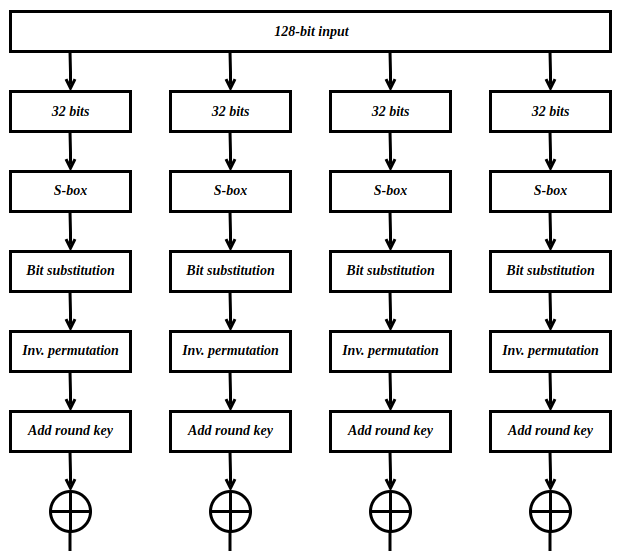
\includegraphics[width=0.8\columnwidth]{figures/GIFT-ROUND.png}
    \caption{Representation of the encryption round function of GIFT\cite{yasmin2023modified}.}
    \label{fig:GIFT-}
\end{figure}

\subsubsection{Reasons for implementation}

The GIFT block cipher, known for its efficiency, has traditionally relied on linear functions within its KSA. However, this approach exhibits vulnerabilities, potentially leading to diminished performance and the predictability of bit transitions. This novel iteration of GIFT proposes the incorporation of bitslice substitution and involutive permutation operations to improve the randomness and diffusion characteristics. These security enhancements to a well-regarded cipher appear to be a promising advancement.

\subsection{SAND}
SAND is a family of two AND-RX block ciphers with Feistel structure, SAND-64, a 64-bit block size, 48-round cipher, and SAND-128, a 128-bit block size, 54-round cipher. Due to its larger block size offering potentially stronger security, SAND-128 will be implemented for this project\cite{SAND}.
\subsubsection{Structure for encryption and decryption}
The round function of the SAND cipher depends on a mix of AND, rotation, and XOR operations. Following the principle of expand-then-compress, the left input branch expands into two branches to facilitate parallel confusion and diffusion within the round function. Each round consists of constant rotation, non-linear functions, bit permutation, an XOR operation with the right input, and the addition of the round key. The decryption process is very similar to encryption, but the round keys are applied in reverse order. This allows the network to reverse the operations performed during encryption and recover the original data. For a detailed breakdown of the encryption process and the complete KSA, refer to the original proposal by Chen et al\cite{SAND}. Refer to Fig.\ref{fig:SAND-} for a representation of the round function.

\begin{figure}
    \centering
    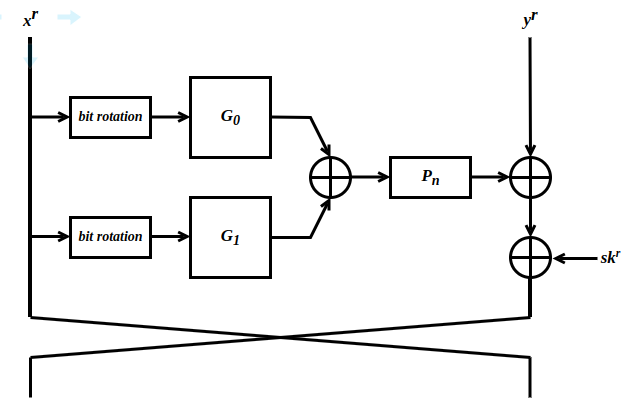
\includegraphics[width=0.9\columnwidth]{figures/SAND-ROUND.png}
    \caption{Representation of the encryption round function of SAND\cite{SAND}.}
    \label{fig:SAND-}
\end{figure}


\subsubsection{Reasons for implementation}
SAND leverages a novel design approach that restricts its AND-RX operations to work within 4-bit nibbles. This unique approach allows SAND to be represented equivalently using a 4x8 synthetic S-box (SSb). This conversion unlocks the advantage of employing established S-box-based security evaluation methods. Furthermore, the authors claim that the inherent bitslice structure combined with AND-RX operations positions SAND among the top contenders for efficient software implementation. The simplicity of employing AND-RX operations and the robustness of well-developed S-box-based security evalution methods and tools appear to be a promising advancement.

\section{Implementation}

This section details the implementation of the SAND-128 and GIFT-128 lightweight ciphers in both software and hardware. The software implementation is carried out in C, while the hardware implementation is performed using Verilog and simulated with ModelSim and QuestaSim. The primary metric used to judge the performance of the hardware implementations is the Gate Equivalent (GE). For the software implementations, execution time, memory usage, and throughput are the key metrics.

\subsection{Software Implementation}

The software implementation involves writing the SAND-128 and GIFT-128 ciphers in C. This subsection describes the process and key considerations for software development.

\subsubsection{Algorithm Specification}

The specifications of SAND-128 and GIFT-128 were studied from their respective academic papers. This study included understanding the key schedule, as well as the encryption and decryption processes.

\subsubsection{Code Development}

Using the algorithm specifications, the encryption and decryption functions for both ciphers were implemented in C. The operations of each cipher, such as substitutions, permutations, key scheduling, and round functions, were translated into C code.

\begin{verbatim}
// GIFT-128 encryption function
void GIFT128_ENC(uint8_t plaintext[16],
                 uint8_t key[16],
                 uint8_t ciphertext[16]){
    // Initialization and key schedule
    // Perform encryption rounds
    // Output ciphertext
}
//
\end{verbatim}

\subsubsection{Testing and Validation}

The implemented C code was tested using test vectors provided in the original cipher specifications and verified against the test vectors in NIST Special Publication 800-38A 2001 ED\cite{dworkin2001recommendation}, which provides recommendations for block cipher modes of operation. The selected encryption mode is the electronic codebook (ECB). The main drawback lies in its limited diffusion capability, as it does not effectively conceal data patterns when encrypting identical plaintext blocks, resulting in identical ciphertext blocks. This critical disadvantage can be ignored when the plaintext blocks are selected in a testing environment, leaving ECB as the optimal encryption mode because of its simplicity. These tests ensured that the software implementation produced correct outputs for known inputs.

\begin{verbatim}
// NIST test vectors
plain-text:
    6bc1bee22e409f96e93d7e117393172a
    ae2d8a571e03ac9c9eb76fac45af8e51
    30c81c46a35ce411e5fbc1191a0a52ef
    f69f2445df4f9b17ad2b417be66c3710
key:
    2b7e151628aed2a6abf7158809cf4f3c
//
\end{verbatim}

\subsubsection{Performance Evaluation}

The performance of the software implementation was evaluated based on the following metrics.

\begin{itemize}
    \item \textbf{Execution Time}: The time taken to perform encryption and decryption operations was measured using high-resolution timers.
    \item \textbf{Memory Usage}: The memory consumption during the encryption and decryption processes was analyzed.
    \item \textbf{Throughput}: The number of operations processed per unit time was calculated to determine the efficiency of the implementation.
\end{itemize}

\subsection{Hardware Implementation}

The hardware implementation of SAND-128 and GIFT-128 was performed using Verilog. The design was simulated using ModelSim and QuestaSim to ensure correctness and performance. The designs were evaluated based on the GEs, which measures the area complexity of the hardware implementation.

\subsubsection{Design Specification}

Similar to the software implementation, the hardware implementation began with a study of the algorithm specifications. This study included understanding the datapath, control logic, and timing requirements of the ciphers.

\subsubsection{Verilog Code Development}

The ciphers were described using Verilog HDL. The design included modules for the key schedule, round functions, and overall control logic.

\subsubsection{Simulation and Verification}

The Verilog designs were simulated using ModelSim and QuestaSim. Testbenches were created to apply test vectors to the design and compare the output with expected results.

\begin{verbatim}
// Testbench for GIFT-128
module GIFT128_Testbench;
    reg [127:0] plaintext;
    reg [127:0] key;
    wire [127:0] ciphertext;

    GIFT128_Encrypt uut (
        .plaintext(plaintext),
        .key(key),
        .ciphertext(ciphertext)
    );

    initial begin
        // Apply test vectors
        plaintext = /* test vector */;
        key = /* test vector */;
        #10; // Wait for encryption 
        $display("Ciphertext: %h",
                 ciphertext);
        // Check if the output matches 
        // the expected result
    end
endmodule
//
\end{verbatim}

\subsubsection{Synthesis and Optimization}

After verifying correctness through simulation, the Verilog code was synthesized using FPGA synthesis tools. This step involved optimizing the design for area and speed, with a focus on minimizing the GEs to ensure a lightweight implementation.


\subsubsection{Implementation on FPGA (not sure)}


\section{Conclusions}
Feistel networks and Substitution-Permutation networks are both fundamental structures for designing lightweight block ciphers. While they share some similarities, they have distinct advantages and disadvantages.

Feistel networks offer inherent invertibility, meaning decryption is straightforward even if the round function itself is not invertible. This simplifies design and analysis. FN ciphers boast several advantages for secure encryption. Each additional round improves the theoretical resistance of the cipher to attacks. Under specific assumptions, their security can be mathematically proven based on the underlying strength of the Feistel function. Additionally, the design offers flexibility by allowing customization of both the Feistel function and the number of rounds to achieve desired security levels. However, these networks also have drawbacks. The overall security hinges heavily on a strong Feistel function, and each round introduces processing overhead, potentially slowing down encryption and decryption.

Substitution-Permutation networks can potentially achieve higher throughput due to their inherent parallelism, making them attractive for hardware implementations with multiple processing units. SPN ciphers are a popular design choice for block ciphers due to their ability to achieve several key security properties.  SPN ciphers achieve confusion by employing S-boxes that perform non-linear operations on the data, making the link between plaintext, key, and ciphertext highly complex. Additionally, P-boxes ensure diffusion by rearranging the data bits, such that a single change in the plaintext has a cascading effect on the final ciphertext. This characteristic, along with the avalanche effect (where minor variations in the plaintext or key lead to significant alterations in the ciphertext), helps resist attacks like differential cryptanalysis. Ultimately, the number of encryption rounds and the design of the S-boxes and P-boxes play a critical role in determining the overall strength and security of an SPN cipher.

Making the best choice between a Feistel network and a Substitution-Permutation network depends on the specific application and design goals. If ease of decryption and hardware limitations are key concerns, a Feistel network might be preferable. If maximizing encryption speed on parallel hardware is a priority, a Substitution-Permutation network might be a better choice.

Additionally, both can be further enhanced with techniques like bit-slicing, custom S-boxes, combined chaotic systems, and even including modifications to the underlying structure to improve security, performance, or both.

Bit-slicing allows for parallel processing on hardware that supports it, potentially leading to significant speed improvements. It is particularly beneficial for lightweight ciphers designed for resource-constrained environments. However, bit-slicing can increase code complexity, so it is important to find a balance between efficiency and implementation effort. Some S-boxes might be designed with low complexity for compact hardware implementations, while others might prioritize high non-linearity for enhanced security.

The development of lightweight cryptography seems to be a continuing search for balance between security and efficiency. On one hand, lightweight ciphers need to be strong enough to resist attacks, but on the other hand, they must also be efficient in terms of resource consumption (memory, processing power) to run on devices with limited capabilities.


\bibliographystyle{IEEEtran}
\bibliography{bibliography/references}
\vspace{12pt}

\end{document}
